%%%%%%%%%% 2. Geometría %%%%%%%%%%%%

\begin{figure}[H]
	\centering
	\includegraphics[scale=0.4]{imagenes/2_geometria_tierra.png}
	\caption{Geometría ingresada con plano a tierra perfecto.}
	\label{fig.geometria_tierra}
\end{figure}

%%%%%%%%%% 3. Diagramas de radiación %%%%%%%%%%

\begin{figure}[H]
	\begin{subfigure}{0.5\textwidth}
		\includegraphics[scale=0.43]{imagenes/2D_80MHz_tierra.png}
	\end{subfigure}	
	\quad
	\begin{subfigure}{0.5\textwidth}
		\includegraphics[scale=0.43]{imagenes/3D_80MHz_tierra.png}
	\end{subfigure}
	\caption{$f=\SI{80}{\mega\hertz}$}
	\label{fig.radiacion_80M_tierra}
\end{figure}


\begin{figure}[H]
	\begin{subfigure}{0.5\textwidth}
		\includegraphics[scale=0.43]{imagenes/2D_160MHz_tierra.png}
	\end{subfigure}	
	\quad
	\begin{subfigure}{0.5\textwidth}
		\includegraphics[scale=0.43]{imagenes/3D_160MHz_tierra.png}
	\end{subfigure}
	\caption{$f=\SI{160}{\mega\hertz}$}
	\label{fig.radiacion_160M_tierra}
\end{figure}


\begin{figure}[H]
	\begin{subfigure}{0.5\textwidth}
		\includegraphics[scale=0.43]{imagenes/2D_240MHz_tierra.png}
	\end{subfigure}	
	\quad
	\begin{subfigure}{0.5\textwidth}
		\includegraphics[scale=0.43]{imagenes/3D_240MHz_tierra.png}
	\end{subfigure}
	\caption{$f=\SI{240}{\mega\hertz}$}
	\label{fig.radiacion_240M_tierra}
\end{figure}


\begin{figure}[H]
	\begin{subfigure}{0.5\textwidth}
		\includegraphics[scale=0.43]{imagenes/2D_320MHz_tierra.png}
	\end{subfigure}	
	\quad
	\begin{subfigure}{0.5\textwidth}
		\includegraphics[scale=0.43]{imagenes/3D_320MHz_tierra.png}
	\end{subfigure}
	\caption{$f=\SI{320}{\mega\hertz}$.}
	\label{fig.radiacion_320M_tierra}
\end{figure}


\begin{figure}[H]
	\begin{subfigure}{0.5\textwidth}
		\includegraphics[scale=0.43]{imagenes/2D_400MHz_tierra.png}
	\end{subfigure}	
	\quad
	\begin{subfigure}{0.5\textwidth}
		\includegraphics[scale=0.43]{imagenes/3D_400MHz_tierra.png}
	\end{subfigure}
	\caption{$f=\SI{400}{\mega\hertz}$.}
	\label{fig.radiacion_400M_tierra}
\end{figure}



\begin{figure}[H]
	\begin{subfigure}{0.5\textwidth}
		\includegraphics[scale=0.43]{imagenes/2D_480MHz_tierra.png}
	\end{subfigure}	
	\quad
	\begin{subfigure}{0.5\textwidth}
		\includegraphics[scale=0.43]{imagenes/3D_480MHz_tierra.png}
	\end{subfigure}
	\caption{$f=\SI{480}{\mega\hertz}$.}
	\label{fig.radiacion_480M_tierra}
\end{figure}	

%%%%%%%%%% 4. CORRIENTES %%%%%%%%%%
\begin{figure}[H]
	\begin{subfigure}{0.5\textwidth}
		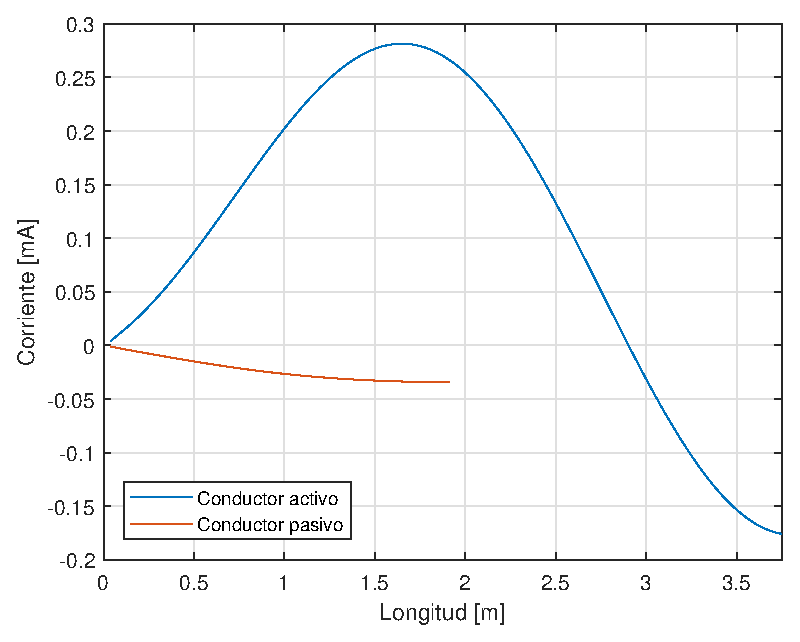
\includegraphics[scale=0.6]{imagenes/i_real_80_tierra.eps}
		\caption{Parte real.}
	\end{subfigure}
	\quad
	\begin{subfigure}{0.5\textwidth}
		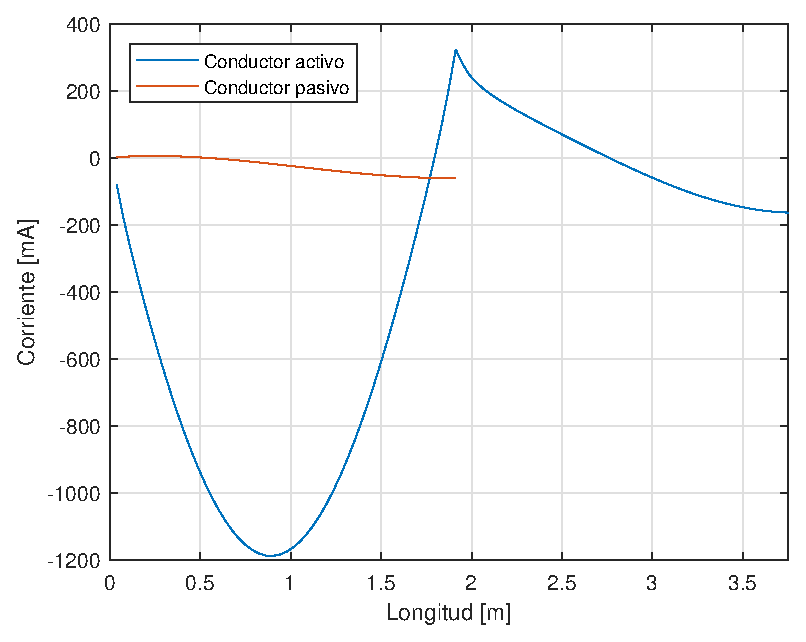
\includegraphics[scale=0.6]{imagenes/i_imag_80_tierra.eps}
		\caption{Parte imaginaria.}
	\end{subfigure}
	\quad
	\begin{subfigure}{0.5\textwidth}
		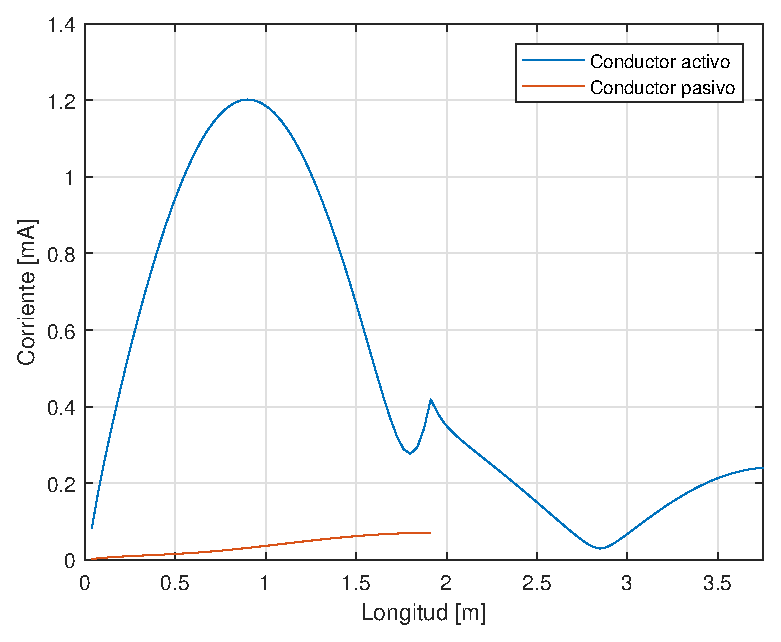
\includegraphics[scale=0.6]{imagenes/i_mag_80_tierra.eps}
		\caption{Magnitud.}
	\end{subfigure}
	\quad
	\begin{subfigure}{0.5\textwidth}
		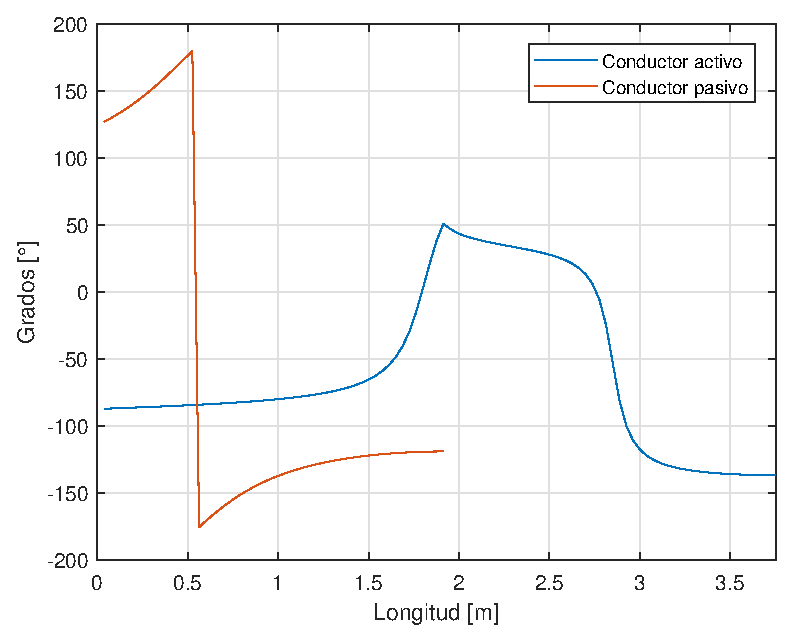
\includegraphics[scale=0.6]{imagenes/i_fase_80_tierra.eps}
		\caption{Fase.}
	\end{subfigure}
	\caption{Corriente para la frecuencia mínima $f = \SI{80}{\mega\hertz}$}
\end{figure}


\begin{figure}[H]
	\begin{subfigure}{0.5\textwidth}
		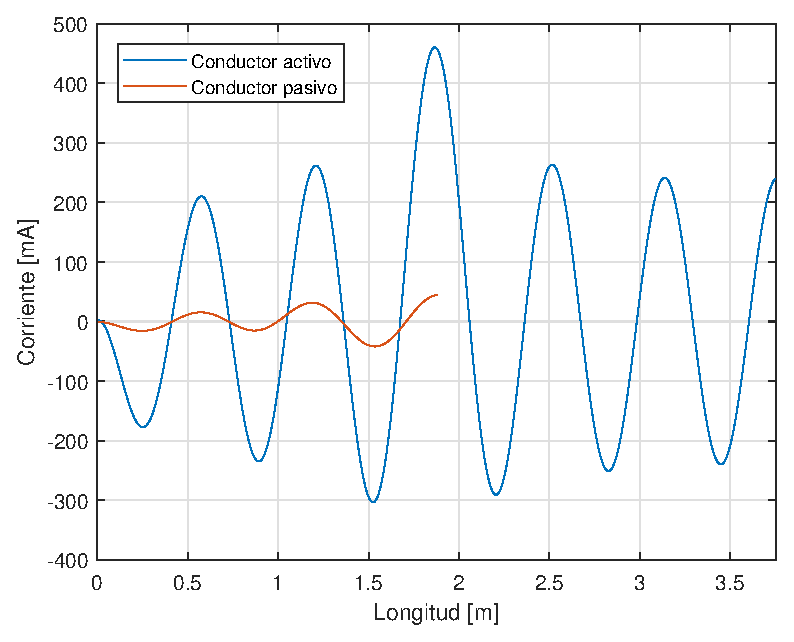
\includegraphics[scale=0.6]{imagenes/i_real_480_tierra.eps}
		\caption{Parte real.}
	\end{subfigure}
	\quad
	\begin{subfigure}{0.5\textwidth}
		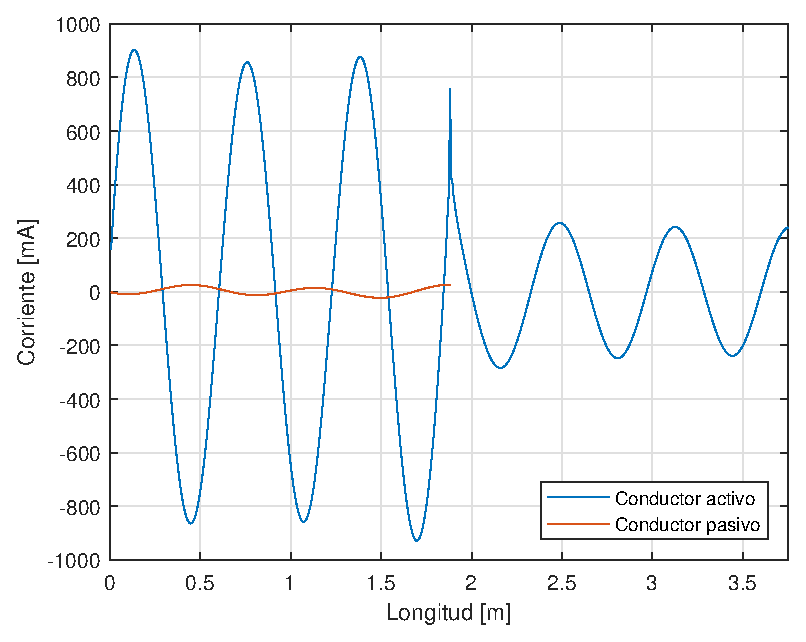
\includegraphics[scale=0.6]{imagenes/i_imag_480_tierra.eps}
		\caption{Parte imaginaria.}
	\end{subfigure}
	\quad
	\begin{subfigure}{0.5\textwidth}
		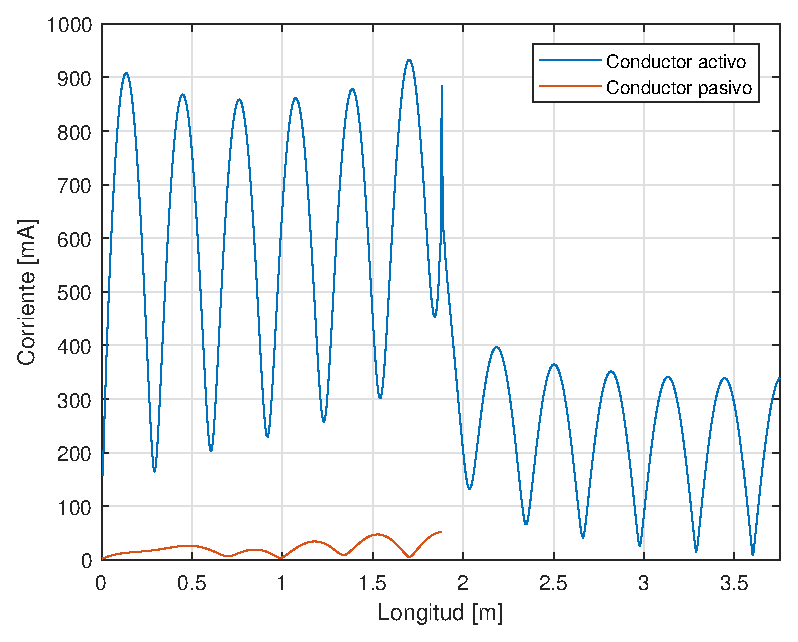
\includegraphics[scale=0.6]{imagenes/i_mag_480_tierra.eps}
		\caption{Magnitud.}
	\end{subfigure}
	\quad
	\begin{subfigure}{0.5\textwidth}
		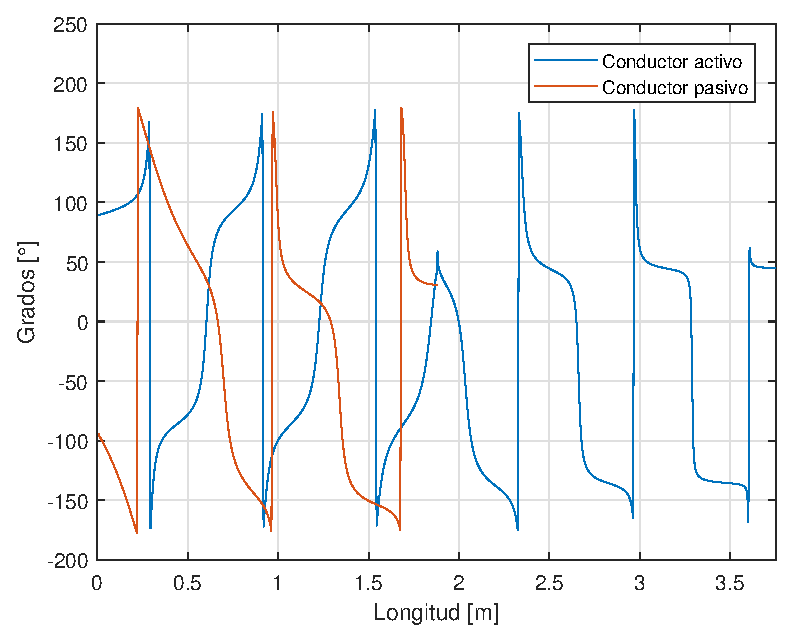
\includegraphics[scale=0.6]{imagenes/i_fase_480_tierra.eps}
		\caption{Fase.}
	\end{subfigure}
	\caption{Corriente para la frecuencia máxima $f = \SI{480}{\mega\hertz}$}
\end{figure}